\chapter{Monitoring native bees}\label{sec:monitoring-native-bees}
\begin{remark}{Outline}
This chapter examines the challenges associated with studies of native bees focusing on the biological field methods typically used to measure species diversity, or populations. A review of conventional techniques is presented by examining two specific approaches for evaluating populations of solitary ground nesting bees using active nest counts.
The use of tools to aid field biology research are introduced, highlighting advances in imaging methods. This chapter summarises the progress of technologies for biological research and presents the validation for an image-centric monitoring method for native bees in New Zealand. This chapter also considers a number of perspectives about the synergy of knowledge between applied science and technology, and the benefits that could arise from the cross-fertilisation of ideas.
\end{remark}

\section{Traditional methods}\label{sec:traditional-methods}
Field research methods which are typically used in biology are often founded on real-world data collections, sampling, measurements or observations. {Field} data can be messy and inexact particularly when compared to the types of data that are acquired using \emph{laboratory} methods. Natural field data sometimes requires special handling  during statistical analyses; especially if it does not conform to assumptions about normality which are required by common statistical techniques. For these reasons considerable care is given to the formation of hypothesis, sampling design and data analysis in studies involving field biology. In the following reviews, methodologies are concerned with multiple species, or groups of insects which are used as indicators of biodiversity. Some studies are specifically designed to measure species diversity while others the population abundance; the methods have or could be used in studies of native bees \footnote{In reference to New Zealand's species, the terms native bees, solitary bees and ground nesting bees are using synonymously throughout the manuscript.}

\subsection{Mark-recapture, survey and passive sampling techniques}\label{sec:mark-recapture,-survey-and-passive-sampling-techniques} 
There are a several techniques that can be used to study insects. However, mark--recapture techniques are considered the most reliable. Because insects are captured using sweep nets, while foraging or above nest sites, some behavioural information can also be gathered. Mark--recapture methods can be used to quantify species diversity and population abundance but they can be labour intensive. They require individual insects to be captured and uniquely marked, then released and caught again. Scientists need expert skills to handle insects and studies are time consuming. In contrast, survey methods are easier to perform. Protocols depend on visual identification of insects in repeat observations of over a pre--determined transect, within a set time--frame. Although surveys are probably less reliable, there are some practical advantages. It is also possible to combine the methods and capitalise on the benefits of both. 

For example, Larsson and Franz \cite{Larson2008} estimated the overall population size of solitary bees by using a small sample of mark--recaptured bees, with an initial observational survey. According to their findings there were good correlations between the methods. They concluded the population size could be reliably established using observational survey walks alone. More importantly they showed their method could save considerable time and effort and thus enable resources to be directed towards long term large scale monitoring. Nonetheless, survey methods are still depend specialist skills and the scientists carrying out observations must be completely familiar with the habitat and bee fauna of survey locations.

Passive sampling methods do not depend heavily on specialist skills so they have some advantages over other techniques. In a comprehensive study, Westphal and Bommarco et al. \cite{Westphal2008} compared a range of sampling methods including: observational plots, pan traps, standardised and variable transect walks and trap nests. Their results showed pan traps were the most efficient and gave the best indication of \emph{species diversity}; similar findings were reported by Nielsen and Steffan--Dewenter et al. \cite{Nielsen2011}. By most accounts pan traps are easy to use and reliable \cite{Westphal2008,Nielsen2011} but others point out they are subject to taxonomic bias \cite{Cane2000,Roulston2007,Tuell2009}. Traps are also fatal for the insects collected, so the method may not be appropriate for research involving vulnerable species? Moreover, several studies have indicated \cite{Cane2000, Wilson2008,Tuell2009} the data gathered from pan traps do not necessarily provide good abundance measurements. They are more suitable for measuring the diversity of species within a habitat.

\subsection{Population methods for solitary bees}\label{sec:population-methods-for-solitary-bees}
Population studies for solitary bees are rare so there are only a few examples to draw upon. In the next few paragraphs two studies are reviewed in turn; the first is by Bischoff \cite{Bischoff2003} and a second, more recent study by Cane \cite{Cane2008}.

In a four year study, Bischoff \cite{Bischoff2003} used mark--recapture and nest counts to evaluate populations of a solitary bee, \emph{Andrena vaga} (Hymenoptera: Andrenidae). Population estimations using nest count data corresponded well with those estimated using mark--recapture data. Bischoff \cite{Bischoff2003} reported little differences between the cumulative number of nests (164) and the mean population estimations (160) for data collected in 1997. He measured an overall decline in the populations of \emph{Andrena vaga} across four years (1996 to 1999) at the sites he monitored. Attributing some of the population changes to corresponding increases in populations of bee parasitoids. Bischoff \cite{Bischoff2003} also concluded mark--recapture methods provided more reliable data.

In an eight year study, Cane \cite{Cane2008} recorded the population changes of the alkali bee, \emph{Nomia melander} (Hymenoptera: Halictidae). Aerial photographs were used to identify fifty--six nest beds across a 240 km$^2$ area of agricultural land. Nest densities were surveyed each year using up to twenty, 1 m$^2$ grids. The grids were scattered randomly on aggregations and the number of nest holes per grid were counted.  Using video recordings, Cane \cite{Cane2008} checked the entry holes that were being actively used by nesting bees, against those counted. He found around 66\% of those manually counted were nest entrances. Consequently, final nest counts were averaged across the total nest area and multiplied by 2/3. Thus accounting for the differences between the observed numbers of nests, with the actual number of nests. Final analysis showed the population density varied within and between nest aggregations. Over the years 1999 to 2006 the population increased by a factor of nine, to an estimated total of 16.7 million.

Taken together the methods used by Bischoff \cite{Bischoff2003} and Cane \cite{Cane2008} support the notion of using nests as a proxy for population abundance. Their studies also highlight the limitations of using nests to estimate absolute population abundances. Manual nests counting methods are likely to produce inflated estimates, at least according to Cane's \cite{Cane2008} experiences. There were instances where several females were using the same entrance to multiple nests underground and other cases indicating solitary females were constructing multiple nests. However, despite these limitations, the number of active nests can provide a broad estimation of the population abundance of solitary ground nesting bees within aggregations; the same method has been successfully used in at least one other study to date \cite{Fellendorf2004}. 

The review also highlighted the paucity of available research. There appears to be a lack of data on the health or populations of many species of solitary bees around the world, not just New Zealand's native bees. In the absence of good data records and with a lack of means to collect any future records, straightforward field methods based on the number of active nests could suffice? At least until alternative field methods have been developed, tested and proved. 


\section{Technologies for field research}\label{sec:technologies-for-field-research}
A diverse range of technological tools are available to science and more are developed each year. According to Moore's Law computing power doubles every eighteen months \cite{Schaller1997,Mack2015} so the rate technological developments and scientific discovery is staggering. Combined with mobile devices, crowd--sourcing projects and increasing connectivity uniting citizen scientists world--wide \cite{Irwin1995}, the volume of data for analysis is changing the scientific landscape. The roadmap is not clearly defined; many studies alter from the traditional knowledge--driven hypothesis testing paradigms to new data--intensive methods \cite{Kelling2009,Catlin2012}. Considering these changes long term meta--analysis of populations of native bees could become a realistic venture within a decade. This review therefore concentrates on tools that are used, or could be used, for field research studies of native bees.

\subsection{Digital tools}\label{sec:digital-tools}
An all purpose recognition tool that can be applied to different classification problems without modification is the goal which challenges most developers today \cite{Mortensen2007,Gaston2004}. Considerable advances have been made to date, but " the bounds on just what it is possible to achieve remain to be established ", as summarised by Gaston and O'Neill \cite[p.12]{Gaston2004}. Automated taxonomic or species identification, refers to computer-based technologies and systems, designed to automatically assign sample specimens into known species using digital data \cite{Gaston2004}. Several formats can be used based on image, audio, or frequency type collections and all have been used in studies for automated identification of insects. This is a rapidly expanding field of research \cite{Macleod2007} typified by exploratory design, therefore some novel studies are presented in this review first. These highlight the advances in digital data analysis, notably the use of audio and frequency--based data and classification methods for insect ID.

The main volume of the review is dedicated to the advances in \emph{imaging systems} since these have revolutionised many scientific studies. Specialised tools have been developed for bees \cite{Roth1999,Arbuckle2001,Steinhage2001}, water insects \cite{Larios2010,Lytle2010}, live moths \cite{Lone2011} and sharks \cite{Towner2013,Van2007}. Combined these studies affirm the \emph{potential} of digital technologies and the benefits that arise from a pooling of resources and knowledge \cite{Kaku1999}. Many frontier projects share common characteristics: they generally involve a range of specialists, methods are developed using open--source tools -- and/or they are designed to be open--access for community science. A selection of representative studies are discussed in the following sections.

\subsection{Audio data}\label{sec:audio-data}
Since insects are more often heard than seen species identification can be difficult. For rapid identification of invertebrates, techniques using digital audio data and frequency--based classifications are most promising as the following studies demonstrate.

Capitalising on the unique acoustic sounds of crickets, Potamitis et al. \cite{Potamitis2006} used audio data for the recognition of \emph{105 different} species.\marginpar{Cricket ID with digital audio data} Their system was based on two main steps; acoustic signal parameterisation and classification. During the first stage they determined the features providing the most information. In the second, they compared the input feature vectors, with a range of predefined models representing target classes. Final results were impressive. They exceeded a 99\% recognition accuracy on the levels of family and subfamily and a 94\% accuracy on the level of \emph{species} \cite{Potamitis2006}.

Raman et al. \cite{Raman2007} developed a low cost acoustic insect flight detector to monitor mosquito activity.\marginpar{Mosquito ID with audio windbeat data} It was constructed using off the shelf components: a noise cancelling microphone and digital sound recorder. They classified recordings using various harmonic ranges of wing--beat frequencies. Pointing out the research behind mosquito identification from audio recordings dates back to 1949's \cite{Offenhauser1949}, Raman et al. \cite{Raman2007} present a system which they report is relatively inexpensive and could realistically perform well in natural environments.

Similarly, Batista et al \cite{Batista2011} developed a low cost optical sensor to count and classify flying insects using wing--beat frequencies. \marginpar{Insect ID with optical wingbeat data} Different species produce distinct wing--beat sounds so they extracted unique acoustic information from recorded sequences. Using Bayesian classification and probabilities they matched wing--beat frequencies with specific species. Large insects produce lower frequencies and smaller insects higher, therefore they suggest classifications are relatively straightforward. They reported an accuracy of 96.04\% using a Bayesian classifier on three different species of insects; including one bumblebee, \emph{Bumble impatiens} (Hymenoptera: Apidae) and two mosquitoes, \emph{Culex quinquefasciatus} and \emph{Aedes aegypti } (Diptera: Culicidae).

\subsection{Image data}\label{sec:image-data}
Caci et al. \cite{Caci2013} used I$^3$S--Contour, Interactive Individual Identification Software\footnote{http://www.reijns.com/i3s/} \cite{Van2007}, to identify individuals belonging to the threatened beetle species \emph{Rosalia alpina} (Coleoptera: Cerambycidae).\marginpar{Beetle image ID and matching with I$^3$S--Contour.} \label{Beetle image ID and matching with I$^3$S--Contour.} Beetles were identified by unique markings on their backs. Selected images were annotated using a semi--automated contour tracing function, matched with unknown images in a reference library and the results given as a ranked picture list. With recognition rates between 94.5--95.2\% (using 290 images) the accuracy of the method was good. Their system could also save time and effort and is perfectly suited for studies concerning vulnerable species. 

In a similar study, Towner et al.\cite{Towner2013} replace mark--recapture with an imaging method to monitor shark populations around the South African coast.\marginpar{Shark image ID and matching with DARWIN.} They used digital images of dorsal fins to identify individual white sharks. They collected images over a four year period (2007 to 2011) and used open--source imaging software DARWIN \cite{Pierrer2006} to process 1683 images of dorsal fins; identifying a total of 532 unique individuals. Their results indicated shark populations had not markedly recovered since being nationally protected by the South African Government in 1991 \cite{Compagno1991}.

Mayo and Watson \cite{Mayo2007} developed an automated species identification system using open--source medical imaging software ImageJ\footnote{ImageJ -- {http://imagej.nih.gov/ij} and FIJI --{http://fiji.sc/Fiji}} \cite{Schneider2012} and {Weka} \cite{Hall2009}. \marginpar{Moth ID with ImageJ \& Weka.} They compared a range of algorithms to automatically classify 35 different species of moths using images of 774 live individuals. They reported an accuracy of 85\% using a support vector machine algorithm, implemented via {Weka}. Likewise, LoNe et al. \cite{Lone2011} developed a real--time image processing system to identify moths in flight in their natural environment. They adapted an algorithm based on randomised trees for training and classification. They achieved an 82\% recognition rate with 10 different species of butterflies.

\section{Relevance of studies}\label{sec:relevance-of-studies}
There are so many different biological methods that can be used to help gather information about native bees \cite{Murray2009}. Only a fraction of these methods have been included in the review. The synthesis was directed towards the methods and tools which could be easily applied or adapted for use, in studies of New Zealand's native bees to increase broad or baseline information about their communities and populations. In the following sections the context of the task is examined closer and in relation to the relevance of the literature reviewed. 

\subsection{Data-intensive science: future field methods?}\label{sec:data-intensive-science:-future-field-methods?}
Multiple disciplines fall within the umbrella of life and natural sciences. Specialists do not always use the same biological methods or field sampling techniques. Consequently, it can be difficult to organise literature into categories for  comparative critique. Therefore it was helpful to categorise studies by using the focus of methodologies which could be aimed towards: 1) a understanding of individuals within a species e.g. Caci et al. \cite{Caci2013}, 2) a selected species group e.g. Towner et al. \cite{Towner2013}, 3) collections of many different species that combine to form communities e.g.Bischoff et al. \cite{Bischoff2003} 4) larger populations of species on a spatio-temporal scale e.g. Cane \cite{Cane2008} 5) or meta-populations or organisms e.g. Murray et. al. \cite{Murray2009}.

Natural science methodologies could also be broadly classed as \emph{observational} or \emph{experimental}. Observed information is nearly always required {before} hypotheses are formed, refined and tested experimentally. The scientific method has changed over time; originating from the emphasis on empirical and observational records to a focus on hypothesis testing and experimental design. Modern research methods which are adopting  data--intensive techniques are fundamentally observational studies \cite{Kelling2009}.
Some of the technologies that are gaining momentum in biology, lend themselves towards meta-data sampling of large populations or communities of species. Kelling et al.\cite{Kelling2009} explored some of the difficulties associated with traditional ecological methods. Since many have been reliant on specialist knowledge and skilled collection techniques, there are some practical and logistical problems when a spatial or temporal understanding of species is required. They point out that well designed, data--intensive research methods can draw on a vast network of human \emph{sensors} \cite{Vitolo2015}. These new approaches can thereby increase data capture for the scientific communities to explore and analyse.

\subsection{Tool selection: what are the criteria?}\label{sec:tool-selection:-what-are-the-criteria?}
There are several specialised tools that work well on a range of target insects that  might not be so easily adapted for use with New Zealand's native bees or their habitats.
Radio telemetry tools \cite{Mascanzoni1986,Lovei1997} were generally excluded from the review even though considerable advances have been achieved in this field over the last decade \cite{Osborne1999,Colpitts2004,Oneil2004}. This is because it is likely that most species of New Zealand's native bees would not carry the added weight of a radio tag. According to a study by Hart \cite{Hart2007} although some species of New Zealand native bees are capable of carrying added loads, they have behavioural characteristics that would precluded the suitability of some tracking technologies. Her observations indicated many species of native bees had behaviours adapted for tunnelling in the soil. They were observed grooming excess dirt from their bodies before attempting flight as shown in Figure \ref{fig:dust}. During load trials she attached added weights to the thorax of bees; in several instances individuals actively manoeuvred into positions in order to dislodge loads \cite[pg. 78]{Hart2007}. For these reasons, automated and semi--automated taxonomic identification tools were considered more appropriate for studies on native bees.

\begin{figure}[!htbp]
\myfloatalign
{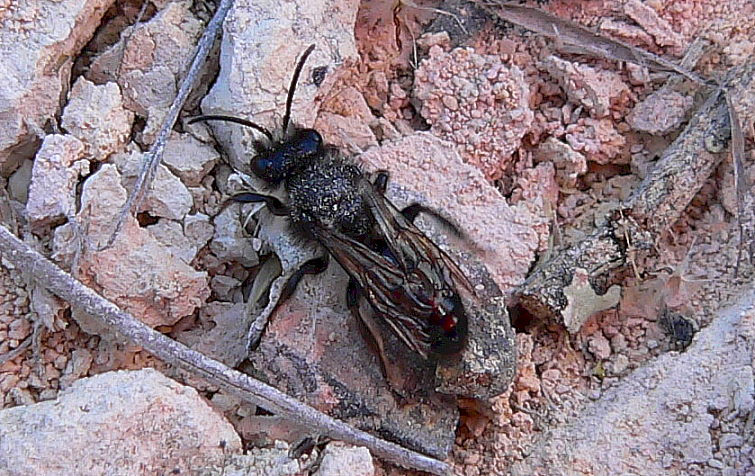
\includegraphics[width=.95\linewidth]{gfx2/bee_dust}} \\
\caption[Female native bee grooming dirt from her body.]{A female native bee has groomed herself to remove clay from her body but some grains remain on her thorax \cite[pg.78]{Hart2007}.}\label{fig:dust}
\end{figure}

\begin{figure}[!htbp]
\myfloatalign
{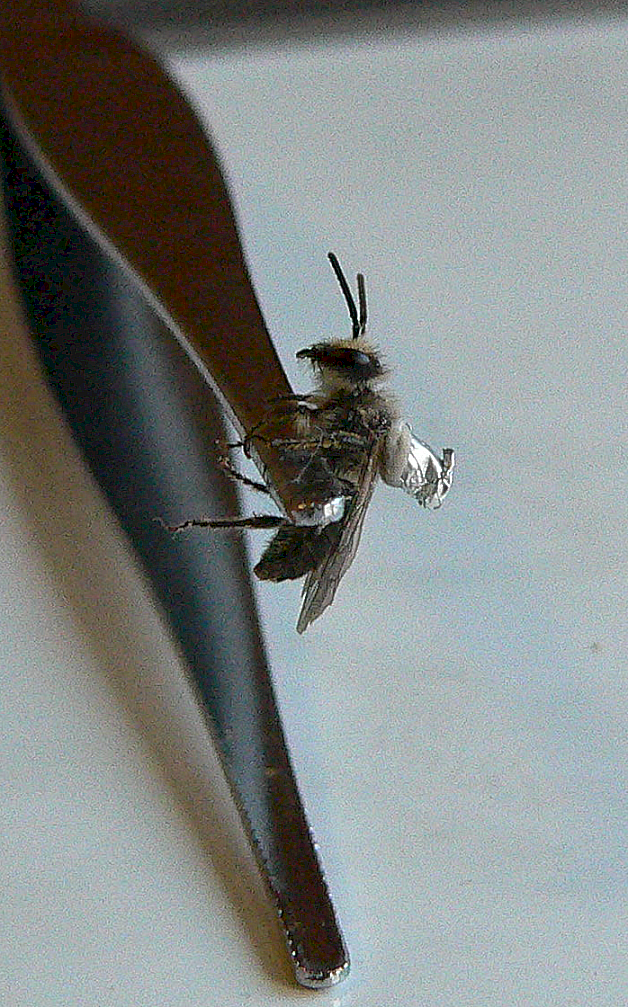
\includegraphics[width=.55\linewidth]{gfx2/bee_load}} \\ 
\caption[Male native bee dislodging load.]{A male native bee attempting to dislodge an artificial load attached to his thorax \cite[pg.78]{Hart2007}.}
\label{fig:track}
\end{figure}

\subsection{Image acquisition: are native bees too small?}\label{sec:image-acquisition:-are-native-bees-too-small?}
A handful of representative studies reviewed thus far are sufficient to demonstrate the range of technologies available. Most are effectively non--invasive mark--release--recapture \emph{type} tools so they are (or could be) used to assess diversity, abundance or behavioural characteristics in a variety of species. This includes New Zealand's native bees. However, there are some aspects, of some imaging tools that would hinder applications for New Zealand's native bees. In the first instance the main issues revolve around the types and qualities of images that can be gathered for analysis. According to Donovan \cite{Donovan2007}, many species of New Zealand's native bees are small compared to other bees. In addition, some closely related species are so morphologically similar they can be difficult to identify properly even using microscopic aids. Previous records collected by Hart \cite{Hart2007} were used to determine the species that were most likely to be found at target the monitoring locations central to this study. These were combined with Donovan's \cite{Donovan2007} research to examine the biometrics of key species in more detail and in relation to current image analysis methods and tools.

The beetle identification system described by Caci et al. \cite{Caci2013} showcases the benefits imaging techniques for studies of vulnerable species. An {image-centric} sampling method is not fatal for target species and therefore has some advantage over traditional methods. However systems using images of target insects might not be easily adapted for monitoring native bees. Acquisition is a problem because of the size and speed of native bees in flight. Also, distinguishing morphological features are usually only perceptible in close-up views. Collecting good scientific sample images of native bees is therefore the main restriction.

A point and shoot approach, using a typical \ac{DSLR} camera can result in some useful scientific images but the method cannot be replicated. As shown in Figure \ref{fig:body} native bees range in body size from around 3--12 mm so if standard images could be collected \emph{size-features} might be useful to classify bees into broad family groups, or even subfamily groups. Native bees are mostly black in colour unlike the target species in the study by Caci et al. \cite{Caci2013}. Compared to the Rosalia longicorn beetle, which is up to 40 mm in body length and has striking physical features (refer to Figure \ref{fig:weevil_beetle} -- b), the differentiating facial characteristics of native bees can only be captured via microscopic-photography as shown in Figure \ref{fig:face}.

If close-up images could be acquired then shape or colour--features from facial markings could be used to identify bees, using any of the analysis methods used by Caci et al. \cite{Caci2013}, Mayo and Watson \cite{Mayo2007} or LoNe et al. \cite{Lone2011}. However, image acquisition would most likely be fatal for the bees, unless they were sedated for close--up imaging and then released \cite{Arbuckle2001}. For a few species, facial features are not significantly different and could not be easily used to differentiate between species. For example, there are no obvious differences between sample images [8] and [10] in Figure \ref{fig:face}. Both are male bees but one belongs to the species \emph{Leioproctus (Leioproctus) huakiwi} (Hymenoptera: Colletidae) and the other to \emph{Leioproctus (Leioproctus) imitatus} (Hymenoptera: Colletidae). 

\begin{figure}[!htbp]
\myfloatalign
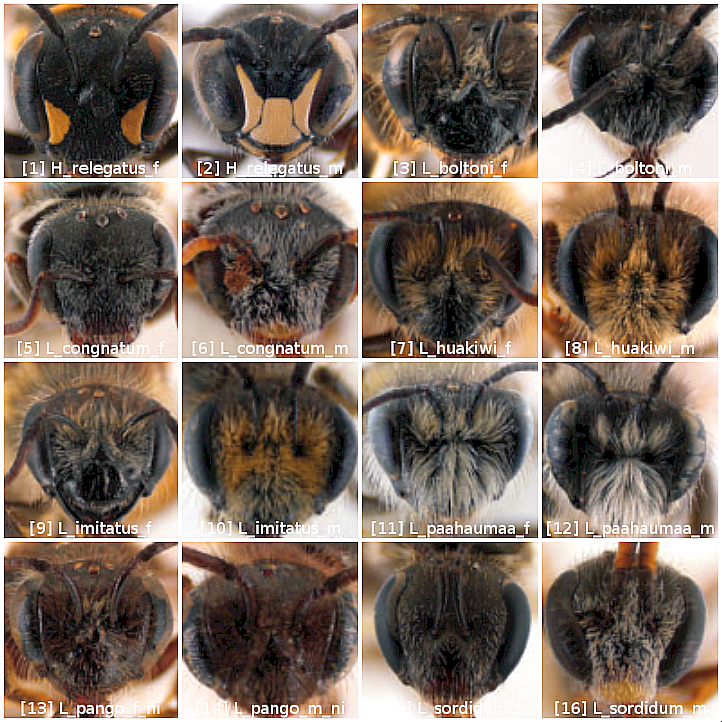
\includegraphics[width=.85\linewidth]{gfx2/bee_face} \\
\caption[The eight species of native bees in Whangarei.]{The eight species of native bees in Whangarei are represented in close-up sample images [1-16]. See \ref{tab:bee_taxa} for species names. Images from Donovan \cite[pp.130--231]{Donovan2007}.} 
\label{fig:face}
\end{figure}

\begin{figure}[!htbp]
\myfloatalign
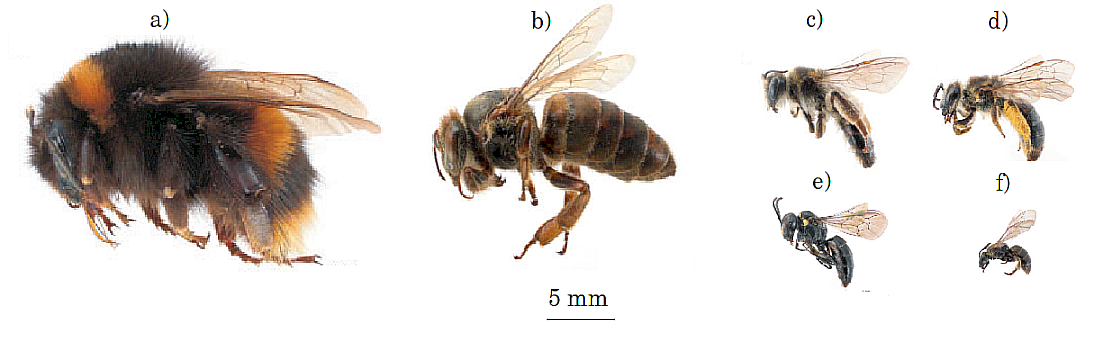
\includegraphics[width=0.85\linewidth]{gfx2/bee_bodies} \\ 
\caption[Bee size to categorise groups.]{Size features could used to categorise bees into broad family groups: such as a) bumble bees, b) honey bees, and c)-f) four\emph{ different} species of native bees. Images from Donovan \cite[pp.130--231]{Donovan2007}.}
\label{fig:body}
\end{figure}

\begin{table} \myfloatalign \caption[Native bees sampled.]{Eight species of native bees have previously sampled in Whangarei \cite{Hart2007}. Based these records the target monitoring locations central to this thesis were likely to have included some of these species. These bees are shown in {Figures} \ref{fig:face} and \ref{fig:body}.}\label{tab:bee_taxa} 
\begin{tabular}{lll}\toprule 
Taxonomic tree & Image reference \\ \midrule
Superfamily APOIDEA \\
Family Colletidae & \\
\ \ \ Subfamily Colletinae & \\
\ \ \ \ Genus Leioproctus & \\
\ \ \ \ Subgenus Leioproctus & \\
\ \ \ \ \ \ \emph{boltoni} & \ \ {\footnotesize [3-4]} {\footnotesize \ref{fig:face}}   \\
\ \ \ \ \ \ \emph{huakiwi} &  \ \  {\footnotesize [7-8]}   \\
\ \ \ \ \ \ \emph{imitatus} & \ \  {\footnotesize [9-10]} & {\footnotesize d)}\female \ {\footnotesize \ref{fig:body}} \\
\ \ \ \ Subgenus Nesocolletes & \\
\ \ \ \ \ \ \emph{paahaumaa} & \ \ {\footnotesize [11-12]} & {\footnotesize c)}\female \\
\ \ \ \ Subfamily Hylaeinae & \\
\ \ \ \ \ \ Genus Hylaeus & \\
\ \ \ \ \ \ Subgenus Prosopisteron & \\
\ \ \ \ \ \ \ \ \emph{relegatus} & \ \  {\footnotesize [11-12]} & {\footnotesize e)}\female \\
\ \ \ \ Subfamily Hylaeinae & \\
\ \ Family Halictidae & \\
\ \ \ \ Subfamily Halictinae & \\
\ \ \ \ Tribe Halictini & \\
\ \ \ \ \ \ Genus Lasioglossum & \\
\ \ \ \ \ \ Subgenus Austrevylaeus & \\
\ \ \ \ \ \ \ \ \emph{sordidum}& \ \  {\footnotesize [15-16]} & {\footnotesize f)}\female \\
\ \ \ \ \ \ Subgenus Chilalictus & \\
\ \ \ \ \ \ \ \ \emph{cognatum }& \ \ {\footnotesize [5-6]}\\
\ \ Family Apidae & \\
\ \ \ \ Subfamily Apinae& \\
\ \ \ \ Tribe Bombini & \\
\ \ \ \ \ \ Genus Bombus & \\
\ \ \ \ \ \ Subgenus Bombus& \\
\ \ \ \ \ \ \ \ \emph{terrestris}& \ \ &{\footnotesize  a)}\female  \\
\ \ \ \ Tribe Apini& \\
\ \ \ \ \ \ Genus Apis & \\
\ \ \ \ \ \ \ \ \emph{mellifera}& \ \ &{\footnotesize  b)}\female \\ \bottomrule
\end{tabular}
\end{table}


\subsection{Image verse audio data?}\label{sec:image-verse-audio-data?}
Image acquisition might not be so challenging in the future, especially as the performance of digital cameras continues to improve. Currently however, without good equipment and stationary target insects, imaging live native bees for scientific analysis is impractical. This is not true for audio data. Theoretically data could be easily collected and an identification system developed to automatically classify native bees into species? The benefits of an insect identification and counting system using digital audio and wing--beat data would be considerable but there is little evidence the tools developed by Potamitis et al. \cite{Potamitis2006}, Raman et al. \cite{Raman2007} and Batista et al. \cite{Batista2011} and have be used in wider monitoring studies. 

This situation might change as the technology becomes more familiar. More so since many of the technologies are being designed for open--access, community--science projects and benefit from crowd--sourced data \cite{Catlin2012,Vitolo2015}. Referring to their insect sensor Batista et al. \cite{Batista2011} explain, "...within the limits of our budget, we will continue our practice of giving a complete system as shown to any research entomologist who requests one..." \cite{Batista2011}. An audio--based identification system for New Zealand's native bees could be worth perusing, particularly for biodiversity studies.

The speed at which new tools and techniques are integrated into ecological methods may be dependent on other intangible factors that may not be easy to overcome? Perhaps more could be achieved towards building greater collaborative relationships across multiple disciplines? Currently, there are many promising technologies have been developed for biological studies (such as those described by \cite{Potamitis2006}, Raman et al. \cite{Raman2007} and Batista et al. \cite{Batista2011}) that do not appear to be utilised? The real benefits of these tools remain largely unknown since they can only be realised when they are incorporated into larger scientific studies. 

\section{Measuring populations using images}
Broad image data, used on a much larger scale, could also help to describe the population dynamics of species over time and space \cite{Kelling2009}. However, there are few exemplar studies in this area and no known research around monitoring the populations of native bees using digital images and image analysis. Nevertheless, the progress of imaging technologies for science is well supported by open--source community initiatives; and there are also some parallel studies with closely related problems and possible solutions. These are presented in the preceding sections.

\subsection{Examining closely related problems}\label{sec:examining-closely-related-problems}
Solis--S{\'a}nchez et al. \cite{Solis2009} developed a machine vision algorithm to detect whiteflies, \emph{Bemisia tabaci} (Homoptera: Aleyrodidae). \marginpar {Whiteflies with digital images.} By taking advantage of the regular shape of whiteflies, they used geometric image features such as solidity, eccentricity and area, to identify whiteflies from other insects caught in traps. They reported a 97--100\% accuracy identifying insects using images of sticky traps and leaves.

They expanded their initial system to identify five different types of insects captured in hunting traps by using their original algorithm, followed by a scale--invariant feature transformation procedure \cite{Solis2011}. Their results showed an improvement on their original system; automatic and manual classifications were highly correlated, returning correlations of between  0.96 -- 0.99 (R$^2$). They point out the benefits for pest management in greenhouse crop production environments, since their system was designed to replace time consuming, labour intensive manual counting methods. While they have much to offer to any research involving technologies for biological field data analysis, their system is based on proprietary software so it is most likely limited to a commercial audience.

Checchi et al. \cite{Checchi2013} presented a method to count the displacement of human populations using high--resolution satellite images. \marginpar{Displaced human populations with satellite images.} They show that digital images are increasingly used in emergency scenarios; for regional level mapping, site planning, vulnerability or damage assessments and in settings to estimate populations sizes. They calculate there are around 43 million people worldwide who are forcibly displaced, due to armed conflict or other crises. Of those populations, at least 33 million remain internally displaced. Another 10 million people are refugees. 

Knowing the size of displaced populations is critically important, especially in the first few days of a disaster. According to Checchi et al. \cite{Checchi2013} good quantitative data is required to help assess any adverse affects on populations; to allocate aid resources effectively, to plan for or and mitigate problems due to the arrival of displaced populations. They use manual identification by counting the number of building structures in images, explaining the results are good enough for estimating human populations. Their method is fit for purpose, especially if there are few alternatives and  a critical time frame. For example, a ground census conducted by human personnel may not be possible during a natural emergency or in a crisis. Moreover, broad, reliable quantitative population data is required as quickly as possible.

In a final related study, Johansson \cite{Johansson2011} also uses satellite imagery for the automatic identification of small marine vessels. \marginpar{Marine vessels with satellite images.} He explains there are increasing levels of piracy on the sea, so detecting and monitoring activities of small vessels is becoming important. Larger ships are regulated and already monitored by automatic identification systems. However, smaller vessels are more difficult to identify, even with the availability of high--resolution satellite data. This is because until recently imaging methodologies have employed thresholding methods to segment image data into key components. 

As with other real--world imaging problems, straightforward segmentation of satellite images into 'vessel' and 'all other objects' is more complex. Satellite images are subjected to natural variations. For example, illumination, brightness and contrast are not necessarily even across an image, so thresholding methods perform poorly. In order to compensate for this, Johansson \cite{Johansson2011} used a specialised filtering technique to highlight objects in images. He used the combined the filtering with a machine learning algorithm, the \emph{Random Forest} and implemented classifications via WEKA\footnote{{http://www.cs.waikato.ac.nz/ml/weka/}}. Johansson \cite{Johansson2011} described his study as novel within the field of vessel detection. Results of the study were exceptional. He achieved an 85--99\% accuracy classifying ships in images obtained from Google Maps. He summarised " as the amount of data increases so does the need for efficient methods of processing such data. " \cite[pg. 1]{Johansson2011}. With such a wealth of digital images now available, he raises a good point.

\section{Review summary}\label{sec:review-summary} 
\begin{remark}{Beyond the data deluge}
Bell et al. \cite{Bell2009} explain, " Over the past 40 years or more, Moore's Law has enabled transistors on silicon chips to get smaller and processors to get faster. At the same time, technology improvements for disks for storage cannot keep up with the ever increasing flood of scientific data generated by the faster computers."  \cite [pg. 1287]{Bell2009}
\end{remark}

According to Bischoff \cite{Bischoff2003} and Cane \cite{Cane2008} it is possible to use the active nests of native bees as a proxy for population abundance. Both studies relied on manual field counting methods; although Cane \cite{Cane2008} used digital video data to confirm the number of active nests (i.e. those nests being used by bees). Manual nest counting methods could be substituted with image-centric techniques. Image acquisition could be easily incorporated into traditional field methods and provide an efficient and reliable method, not heavily dependent on expert manual field protocols. 

The future prospects of automated taxonomic identification from images for native bees is promising. But there are practical constraints associated the biology and behaviour of many native species that limits acquisition of good scientific images.  At least where images of live insects are concerned. It may also be possible to sedate or fix insects for image acquisition, as Arcuckle et al. \cite{Arbuckle2001} do in their automated bee identification system (ABIS). However, the extra tools \footnote{Such as laptop, dissecting microscope, macro lens and flash lighting equipment}, time and effort required may defeat the purpose, at least in terms of the aims of this thesis. This is equally true for audio--based collections, since most are used for species identification and not aimed at collecting rapid broad, spatio temporal population data (Section \ref{sec:audio-data}). The objective of this thesis is to collect reliable base-line information on the health of native bee communities, therefore a \emph{simplified monitoring} method is paramount. The techniques outlined in this thesis could also be viewed as first line tools, highlighting potential population changes and identifying locations where more in depth diversity research is needed.

Once image data has been reliably collected, image collation, management and analysis choices and tasks become central. As Hey \cite{Hey2009} explains, " People are collecting data either from instruments or sensors, or from running simulations. Pretty soon they end up with millions of files, and there is no easy way to manage or analyze their data." \cite{Hey2009}. Data--intensive research brings much opportunities and great challenges \cite{Kelling2009, Goodchild2010}. The ways to handle and process vast amounts of information to provide useful results are not always as easily defined as expressed by Johansson \cite{Johansson2011}; similar concerns are echoed by many others \cite{Kelling2009, Hey2009, Lindenmayer2013}. Certainly there are rapid swings and gains in scientific knowledge \cite{Sanchez2011}. Technologies continually improve in performance and power, doubling every year \cite{Mack2015}. Increasing connectivity unties large networks of human sensors \cite{Goodchild2007} as e-science rapidly replaces traditional empirical methods \cite{Hey2009, Bell2009}.

Many more organisations recognise the benefits of interdisciplinary research\label{socially relevant science}; the cross pollination and ideas that emerge from a synergy of different skills and perspectives, that enrich discovery \cite{Kaku1999}. But as Hampton et al.\cite{Hampton2013} acknowledge, " The scientists who contribute such information will be at the forefront of socially relevant science -- but will they be ecologists? " \cite[pg. 156]{Hampton2013}. Possibly not, since while other scientific fields embrace the era of big data, many branches of ecology are slow to move toward more open models of research \cite{Hampton2013}. At the other end of this argument, Lindenmayer and Likens\cite{Lindenmayer2013} point out, "...in our discipline of ecology, there is an increasing number of examples where increased knowledge is missed or even where substantially flawed papers are being published, in part because authors had limited or no understanding of the data sets they were using, nor any experience of the ecosystems or other entities about which they have written." \cite[pg. 338]{Lindenmayer2013}. 

Certainly both perspectives have merit, at least with regards to this thesis, which presents an image--centric system intended for practical applications in biological science -- to monitor spatio temporal changes in populations of New Zealand's native bees using images of active nests and semi-automated image analysis. Without doubt this thesis would not meet the criteria for rigorous scientific analysis.  However the image--centric techniques presented do demonstrate the potential use in future monitoring. If the tools were used as part of a wider monitoring programme, the data could contribute to a greater understanding of native bees and their ecosystems. This could be a vast improvement on the current state of knowledge.

Interesting points were raised by Hampton et al. \cite{Hampton2013}, Lindenmayer and Likens \cite{Lindenmayer2013} as they both elucidate the current issues affecting ecological research. In other areas of natural science, open access, big data archiving and sharing, image processing and analysis, machine learning and data mining, and e--science have been integrated into methods.  Biomedical imaging research collaborations have culminated in dynamic and useful open source tools, such as \ac{Fiji} and ImageJ \cite{Schneider2012}. But there are no such clear paths for many ecological studies and a limited number of examples to draw upon for inspiration. This is somewhat the case in this thesis, as there are no know examples, either in New Zealand or abroad, where images have been used to monitor populations of ground nesting solitary bees.

There is some inspiration found in a wider domain by looking at similar problems and parallel studies. Therefore in the final sections of this review a number of analogous studies were reviewed. By evaluating representative imaging methods and closely related studies, the probability image--centric techniques could be successfully applied in studies of native bees is established. However, in order to implement the many other specific aspects of this method (i.e. image storage, archiving and analysis), biomedical imaging research often provides some of the best methodological examples to follow. The advances in biomedical imaging systems have had a significant impact in the fields of human biology and medicine. They can also be applied to a range of other life--science research and have provided the foundation for other novel image--centric studies. These are introduced in the next chapter with a review of the developments in open--source imaging systems. 

\begin{figure}[!htbp]
\myfloatalign
{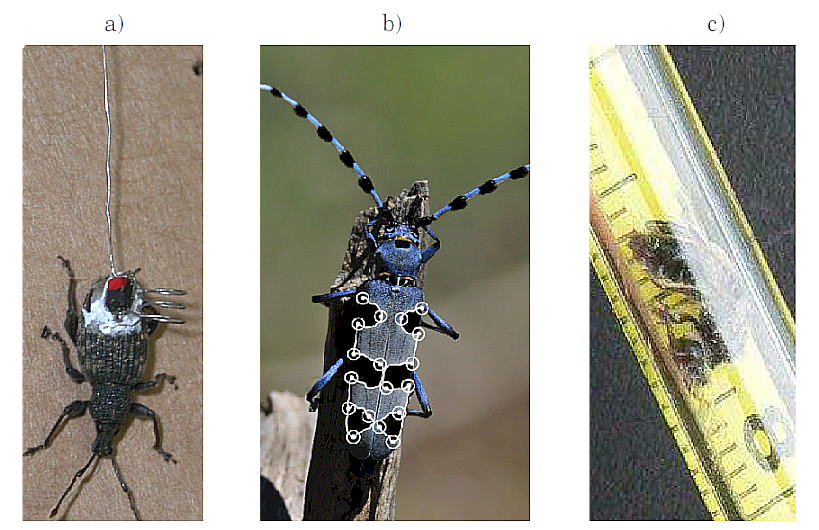
\includegraphics[width=0.85\linewidth]{gfx2/weevil_beetle}}
\caption [Harmonic radar and I$^3$S-Contour.]{From Barzee et al. \cite{Brazee2005} a) Harmonic radar transponder attached to a weevil, Caci et al. b) I$^3$S-Contour annotations on the longhorn beetle \cite[pg.788]{Caci2013} and Hart \cite[pg.78]{Hart2007} d), A native bee \emph{turning around} inside a 5 mm wide tube.} \label{fig:weevil_beetle}
\end{figure}

\begin{figure}[!htbp]
\myfloatalign
{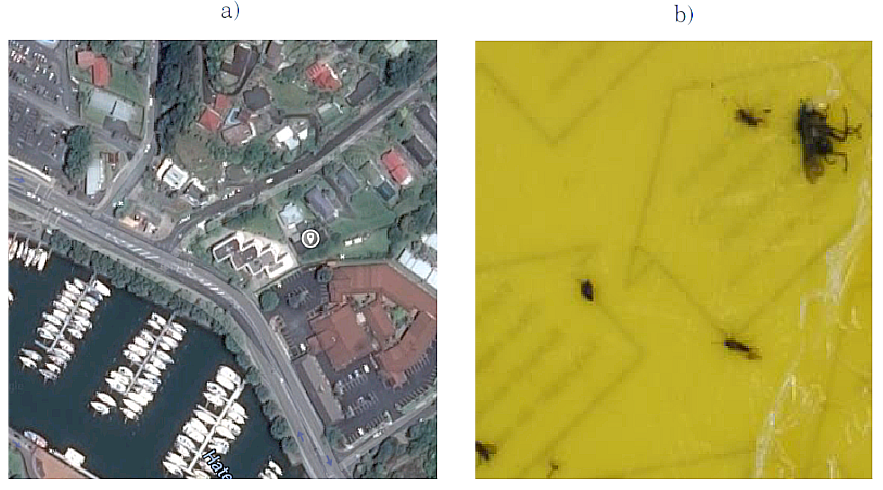
\includegraphics[width=.95\linewidth]{gfx2/sat_boat}} \\ 
\caption [Parallel imaging problems.]{Parallel imaging problems. a) Image of Whangarei (\copyright Google Maps) similar to those used by Checchi et al. \cite{Checchi2013} and Johansson \cite{Johansson2011} and b) Image of a sticky trap similar to those used by Solis--S{\'a}nchez et al. \cite{Solis2009} }\label{fig:sat_boat}
\end{figure}
\clearpage

